\chapter{Lezione 3}
\label{chap:lezione_03} 

\begin{flushright}
\textit{Data: 08/10/2025}
\end{flushright}


\section{Funzione di Cramer per una Variabile Binaria}

Consideriamo una variabile binaria $x$ che può assumere i valori $+1$ e $-1$ con probabilità $1/2$.
\begin{equation}
x = \begin{cases}
+1 & \text{con } p = 1/2 \\
-1 & \text{con } p = 1/2
\end{cases}
\end{equation}

La funzione di Cramer $I(\lambda)$, che caratterizza le grandi deviazioni della somma di $N$ di tali variabili, può essere calcolata. L'espressione iniziale che si ottiene tramite la trasformata di Legendre è:
\begin{equation}
I(\lambda) = \lambda \, \text{arctanh}(\lambda) - \log(\cosh(\text{arctanh}(\lambda)))
\end{equation}

Sfruttando le proprietà delle funzioni iperboliche, questa espressione può essere riscritta in una forma molto più simmetrica e interpretabile:
\begin{equation}
I(\lambda) = \frac{1+\lambda}{2} \log(1+\lambda) + \frac{1-\lambda}{2} \log(1-\lambda)
\end{equation}

Questa forma può essere ulteriormente espressa in relazione a una quantità di tipo entropico. Possiamo scrivere:
\begin{equation}
I(\lambda) = \log(2) - S(\lambda)
\end{equation}
dove $S(\lambda)$ è l'entropia di una variabile di Bernoulli che assume due valori con probabilità $p_1 = \frac{1+\lambda}{2}$ e $p_2 = \frac{1-\lambda}{2}$:
\begin{equation}
S(\lambda) = -\frac{1+\lambda}{2} \log\left(\frac{1+\lambda}{2}\right) - \frac{1-\lambda}{2} \log\left(\frac{1-\lambda}{2}\right)
\end{equation}
È ragionevole che la funzione di Cramer sia legata all'opposto dell'entropia: dove l'entropia è grande (massima incertezza, $\lambda=0$), la funzione di Cramer è piccola (minima), indicando che il valore medio è il più probabile. Viceversa, dove l'entropia è piccola (vicino a $\lambda = \pm 1$), la funzione di Cramer è grande, indicando che le deviazioni estreme sono improbabili.

Il grafico di $I(\lambda)$ in funzione di $\lambda$ è una curva convessa, con un minimo in $\lambda=0$ dove vale zero. Ai bordi del dominio, per $\lambda \to \pm 1$, la funzione tende a $\log(2)$.


\begin{figure}[h!]
\centering
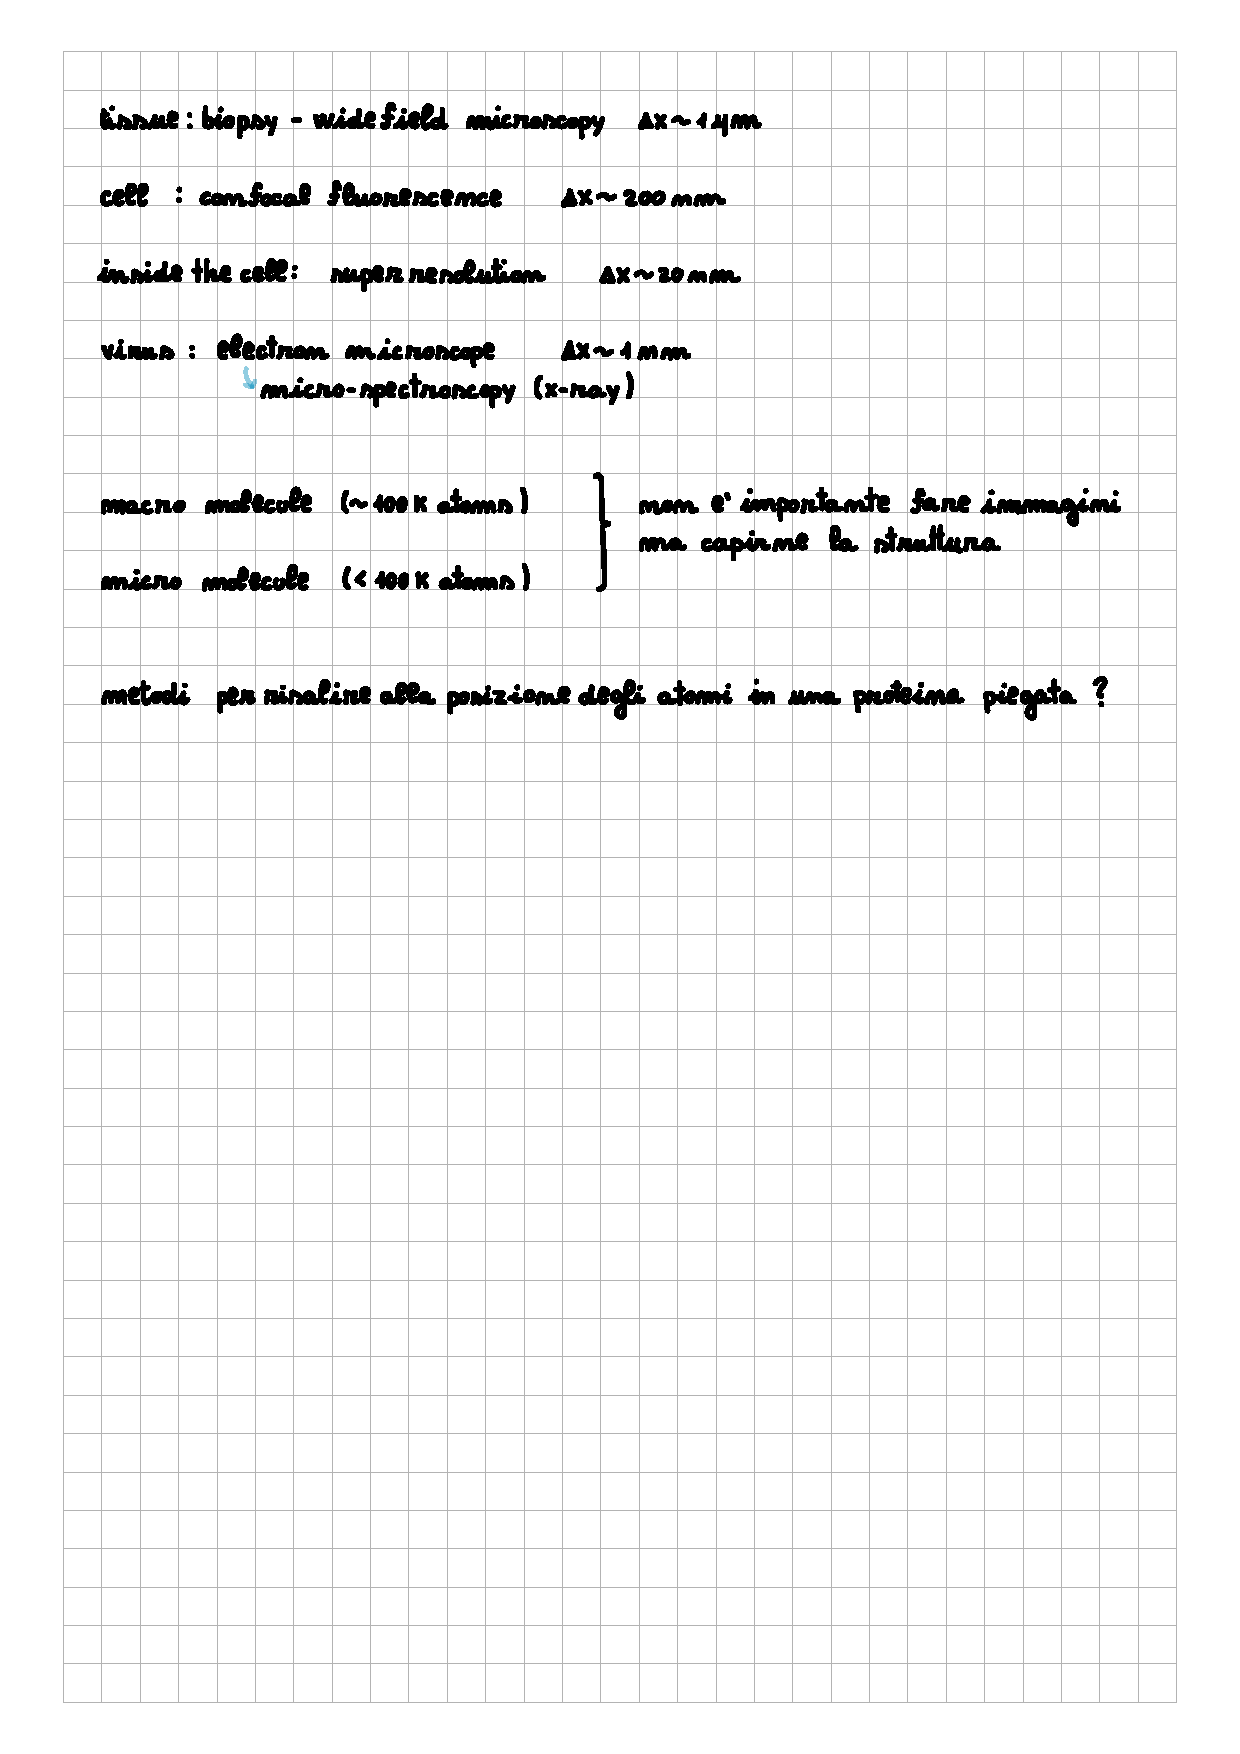
\includegraphics[width=0.5\textwidth]{pics/04.png}
\caption{$I(\lambda)$ in funzione di $\lambda$}
\end{figure}

\noindent Nell'intorno di $\lambda=0$, la funzione può essere approssimata da una parabola $I(\lambda)~\approx~\lambda^2/2$. Questo risultato è coerente con il Teorema del Limite Centrale: la somma di variabili con valore di aspettazione nullo e varianza unitaria tende a una distribuzione gaussiana.

La convessità della funzione di Cramer è una proprietà cruciale per le somme di variabili indipendenti. Essa garantisce l'esistenza di un unico minimo, e quindi di un unico valore più probabile (tipico) per la media campionaria. Allontanandosi da questo valore, la probabilità di osservare una certa media decade esponenzialmente in $N$. Questa caratteristica fondamentale viene a mancare quando si considerano variabili correlate, che è l'argomento che affronteremo ora. Il mondo non è fatto di variabili indipendenti, e la principale conseguenza della correlazione è la possibile perdita di convessità, che porta alla comparsa di più minimi per la funzione di Cramer.

\newpage
\section{Introduzione alle Variabili Correlate}

Per descrivere un sistema di due variabili correlate, $X$ e $Y$, è necessario utilizzare la \textbf{distribuzione di probabilità congiunta}, $P_{X,Y}(x, y)$. Per semplicità di notazione, la indicheremo come $P(x,y)$.

A partire dalla distribuzione congiunta, si possono definire altre due distribuzioni fondamentali.


Le \textbf{distribuzioni marginali} si ottengono "integrando via" (o sommando, nel caso discreto) le altre variabili. Forniscono la distribuzione di probabilità di una singola variabile, indipendentemente dal valore delle altre.
\begin{equation}
P_X(x) = \sum_y P(x,y)
\end{equation}
\begin{equation}
P_Y(y) = \sum_x P(x,y)
\end{equation}

Le \textbf{distribuzioni condizionali} descrivono la probabilità di una variabile, dato che un'altra variabile ha assunto un valore specifico. La distribuzione congiunta può essere fattorizzata in due modi equivalenti:
\begin{equation}
P(x,y) = P_{Y|X}(y|x) P_X(x) = P_{X|Y}(x|y) P_Y(y)
\end{equation}
Questo significa che per generare una coppia $(x,y)$ si può prima estrarre $x$ dalla sua marginale $P_X(x)$ e poi, condizionatamente al valore di $x$ ottenuto, estrarre $y$ da $P_{Y|X}(y|x)$, o viceversa.


Uguagliando le due espressioni per la probabilità congiunta, si ottiene immediatamente il \textbf{Teorema di Bayes}:
\begin{equation}
P_{X|Y}(x|y) = \frac{P_{Y|X}(y|x) P_X(x)}{P_Y(y)}
\end{equation}

Questa formula, sebbene sia una semplice identità matematica, assume un significato profondo quando si passa dal concetto di \textbf{correlazione} a quello di \textbf{causalità}. È un principio fondamentale da tenere sempre a mente: \textbf{correlazione non implica causalità}. Il fatto che due eventi siano statisticamente correlati non significa che uno sia la causa dell'altro. Esistono innumerevoli esempi di "correlazioni spurie", in cui due serie di dati mostrano andamenti quasi identici pur essendo causalmente slegate.

Il Teorema di Bayes acquista il suo potere inferenziale quando si ipotizza un modello causale, ad esempio che una variabile $X$ (la causa) influenzi una variabile $Y$ (l'effetto). In questo contesto, i termini del teorema assumono un'interpretazione fisica precisa:
\begin{itemize}
    \item $P_{X|Y}(x|y)$ è la \textbf{distribuzione a posteriori}: la probabilità (o la nostra credenza) sulla causa $x$ dopo aver osservato l'effetto $y$.
    \item $P_X(x)$ è la \textbf{distribuzione a priori} (o \textit{prior}): la nostra conoscenza o aspettativa sulla variabile $X$ prima di effettuare qualsiasi misura su $Y$.
    \item $P_{Y|X}(y|x)$ è la \textbf{verosimiglianza} (o \textit{likelihood}): questa è la probabilità condizionata "in avanti", che descrive come la causa $x$ produce l'effetto $y$. Questo termine incapsula il nostro \textbf{modello} del processo fisico.
    \item $P_Y(y)$ è un termine di normalizzazione (l'\textit{evidence}).
\end{itemize}
L'inferenza bayesiana consiste quindi nell'utilizzare un'osservazione ($y$) e un modello ($P_{Y|X}(y|x)$) per aggiornare la nostra conoscenza su una causa non osservata ($x$), passando dalla distribuzione a priori a quella a posteriori.



Se le variabili $X$ e $Y$ sono indipendenti, l'intero formalismo si semplifica notevolmente. La condizione di indipendenza è che la distribuzione congiunta si fattorizzi nel prodotto delle marginali:
\begin{equation}
P(x,y) = P_X(x) P_Y(y)
\end{equation}
Di conseguenza, le distribuzioni condizionali diventano indipendenti dalla variabile condizionante:
\begin{equation}
P_{Y|X}(y|x) = P_Y(y)
\end{equation}
\begin{equation}
P_{X|Y}(x|y) = P_X(x)
\end{equation}

\subsection{Entropia e Informazione Mutua}

A ogni distribuzione di probabilità possiamo associare un'entropia di Shannon, che misura l'incertezza o la quantità di informazione.

\begin{itemize}
    \item \textbf{Entropia Congiunta}: Misura l'incertezza totale della coppia di variabili $(X,Y)$.
    \begin{equation}
    H_{X,Y} = -\sum_{x,y} P(x,y) \log P(x,y)
    \end{equation}
    
    \item \textbf{Entropia Condizionale}: Misura l'incertezza media residua su $Y$ quando il valore di $X$ è noto. Si calcola mediando l'entropia di $P_{Y|X}(y|x)$ su tutti i possibili valori di $x$.
    \begin{equation}
    H_{Y|X} = -\sum_x P_X(x) \sum_y P_{Y|X}(y|x) \log P_{Y|X}(y|x)
    \end{equation}
    
    Queste quantità sono legate dalla \textbf{regola della catena} (\textit{chain rule}) per l'entropia:
    \begin{equation}
    H_{X,Y} = H_X + H_{Y|X}
    \end{equation}
    L'incertezza totale è la somma dell'incertezza su $X$ più l'incertezza residua su $Y$ una volta noto $X$.
\end{itemize}

Per quantificare in modo simmetrico l'informazione condivisa tra due variabili, si introduce l'\textbf{Informazione Mutua} (\textit{Mutual Information}), una quantità fondamentale nell'analisi dati e nell'inferenza.

\begin{equation}
I_{X,Y} = \sum_{x,y} P(x,y) \log \frac{P(x,y)}{P_X(x) P_Y(y)}
\end{equation}

Questa quantità è la divergenza di Kullback-Leibler tra la distribuzione congiunta $P(x,y)$ e la distribuzione che le variabili avrebbero se fossero indipendenti, $P_X(x) P_Y(y)$. Quindi, $I_{X,Y} = D_{KL}(P(x,y) || P_X(x) P_Y(y))$.

Proprietà fondamentali:
\begin{itemize}
    \item $I_{X,Y} \ge 0$.
    \item $I_{X,Y} = 0$ se e solo se $X$ e $Y$ sono indipendenti.
\end{itemize}

L'informazione mutua può essere espressa in termini di entropie, rivelandone il significato intuitivo:
\begin{equation}
I_{X,Y} = H_Y - H_{Y|X} = H_X - H_{X|Y}
\end{equation}
Essa rappresenta la \textbf{riduzione dell'incertezza} su una variabile (es. $H_Y$) che si ottiene grazie alla conoscenza dell'altra (misurata dall'incertezza residua $H_{Y|X}$). Se le variabili sono perfettamente correlate (es. $Y=f(X)$), allora $H_{Y|X}=0$ e $I_{X,Y}=H_Y$: conoscere $X$ rimuove tutta l'incertezza su $Y$.

\vspace{2cm}
\section*{Dalla Statistica Classica alla Meccanica Statistica in Alta Dimensione}

La statistica classica si occupa tipicamente di sistemi con un numero basso di variabili. Quando il numero di variabili $N$ diventa molto grande ($N \gg 1$), si entra nel campo della \textit{High-Dimensional Statistics}. In questo regime, molti metodi classici falliscono (la cosiddetta "maledizione dell'alta dimensionalità", \textit{curse of dimensionality}), ma emergono nuovi fenomeni collettivi che possono essere studiati con gli strumenti della meccanica statistica.

Per i fisici statistici, l'alta dimensionalità è una "benedizione" (\textit{blessing of dimensionality}), perché nel limite $N \to \infty$ (limite termodinamico) le fluttuazioni si riducono e le quantità macroscopiche si concentrano attorno ai loro valori medi, rendendo i calcoli analitici possibili e predittivi. L'intuizione geometrica cambia radicalmente: per esempio, una distribuzione gaussiana $N$-dimensionale, che in bassa dimensione ha la sua massima probabilità nell'origine, in alta dimensione concentra quasi tutta la sua massa su un guscio sferico a distanza $\sqrt{N}$ dall'origine.

\newpage
\section{Il Modello di Ising}

Il modello di Ising è il modello archetipico per lo studio di un gran numero di variabili binarie interagenti. Fu proposto da Wilhelm Lenz e studiato dal suo dottorando Ernst Ising nel 1923 per descrivere il fenomeno del ferromagnetismo.



Consideriamo un insieme di $N$ variabili binarie $S_i \in \{-1, +1\}$, chiamate \textbf{spin}, disposte sui vertici di un grafo $G=(V, E)$. L'energia del sistema, descritta dall'Hamiltoniana, è data da:
\begin{equation}
H(\underline{S}) = -J \sum_{(i,j) \in E} S_i S_j - h \sum_{i \in V} S_i
\end{equation}
dove:
\begin{itemize}
    \item Il primo termine descrive l'interazione a coppie tra spin connessi da un arco del grafo. $J$ è la \textbf{costante di accoppiamento}. Se $J>0$ (\textbf{ferromagnetico}), lo stato di minima energia è quello in cui gli spin sono allineati ($S_i S_j=1$), favorendo l'ordine.
    \item Il secondo termine descrive l'interazione degli spin con un \textbf{campo magnetico esterno} $h$. Lo stato di minima energia favorisce l'allineamento degli spin con il campo.
\end{itemize}

Il comportamento del modello dipende crucialmente dalla \textbf{topologia} del grafo (catena 1D, reticolo quadrato 2D, ecc.) e dalla sua \textbf{dimensione} $D$. Per i reticoli regolari, si definiscono due dimensioni critiche:
\begin{itemize}
    \item \textbf{Lower Critical Dimension (LCD)}: È la dimensione minima al di sotto della quale non può esistere una transizione di fase a temperatura finita. Per il modello di Ising, $LCD=1$.
    \item \textbf{Upper Critical Dimension (UCD)}: È la dimensione al di sopra della quale il comportamento critico del sistema diventa indipendente dalla dimensione e viene descritto correttamente dalla teoria di campo medio. Per il modello di Ising,~$UCD~=~4$.
\end{itemize}

\subsection{Il Modello di Ising Unidimensionale (1D)}

Ising, nella sua tesi, risolse il modello su una catena lineare ($D=1$), trovando che non presenta una transizione di fase a $T>0$, un risultato deludente che lo portò a concludere erroneamente che il modello non potesse descrivere il ferromagnetismo e ad abbandonare la fisica.

L'Hamiltoniana 1D con interazioni ai primi vicini è:
\begin{equation}
H(\underline{S}) = -J \sum_{i} S_i S_{i+1} - h \sum_i S_i
\end{equation}
Le \textbf{condizioni al contorno} sono importanti:
\begin{itemize}
    \item \textbf{Open Boundary Conditions (OBC)}: La catena è aperta. La somma sulle interazioni va da $i=1$ a $N-1$.
    \item \textbf{Closed/Periodic Boundary Conditions (CBC)}: La catena è chiusa ad anello, con $S_{N+1} \equiv S_1$. La somma va da $i=1$ a $N$.
\end{itemize}
Nel limite termodinamico ($N \to \infty$), le due condizioni portano agli stessi risultati per le grandezze intensive.

\begin{figure}[h!]
\centering
\includegraphics[width=0.6\textwidth]{pics/05.png}
\caption{Modello di Ising 1D.}
\end{figure}

\subsubsection{Risoluzione del Modello di Ising 1D}

Risolvere un modello di meccanica statistica significa calcolare la sua \textbf{funzione di partizione} $Z$ nell'insieme canonico.
\begin{equation}
Z = \sum_{\{\underline{S}\}} e^{-\beta H(\underline{S})}
\end{equation}
dove $\beta = 1/T$ (poniamo $k_B=1$) e la somma è su tutte le $2^N$ configurazioni di spin.

Da $Z$ si deriva l'\textbf{energia libera di Helmholtz} $F = -T \log Z$. 

Poiché $Z \propto e^N$ e $F \propto N$, si lavora con l'energia libera intensiva $f = F/N$, che è una quantità di ordine 1 nel limite termodinamico. Tutte le grandezze termodinamiche si ottengono derivando $f$ rispetto ai parametri esterni ($\beta$ e $h$):

\begin{tcolorbox}[colback=yellow!30,  
                  colframe=yellow!50!orange,  
                  boxrule=0.8pt, 
                  arc=3pt,  
                  top=4pt, bottom=4pt, left=6pt, right=6pt,
                  enhanced,
                  sharp corners=south]
\begin{itemize}
    \item \textbf{Energia libera intensiva}: $f(\beta, h) = -\frac{1}{N \beta} \log Z$
    \item \textbf{Energia interna}: $\epsilon = \frac{\langle H \rangle}{N} = \frac{\partial (\beta f)}{\partial \beta} = f + \beta \frac{\partial f}{\partial \beta}$.
    \item \textbf{Entropia}: $S = \beta^2 \frac{\partial f}{\partial \beta}$.
    \item \textbf{Magnetizzazione}: $m = \frac{\langle \sum_i S_i \rangle}{N} = -\frac{\partial f}{\partial h}$.
    \item \textbf{Suscettività magnetica}: $\chi_m = \frac{\partial m}{\partial h} = -\frac{\partial^2 f}{\partial h^2}$.
\end{itemize}
\end{tcolorbox}


\subsubsection{Calcolo della Funzione di Partizione (con h=0)}

Consideriamo il caso $h=0$.
\begin{equation}
Z = \sum_{\{\underline{S}\}} e^{\beta J \sum_i S_i S_{i+1}} = \sum_{\{\underline{S}\}} \prod_i e^{\beta J S_i S_{i+1}}
\end{equation}

Utilizziamo la seguente identità:


\begin{tcolorbox}[colback=red!15,  
                  colframe=red!40!orange,  
                  boxrule=0.8pt, 
                  arc=3pt,  
                  top=4pt, bottom=4pt, left=6pt, right=6pt,
                  enhanced,
                  sharp corners=south]
\begin{equation}
    e^{AS} = \cosh(A) [1 + S \tanh(A)]
\end{equation}
\end{tcolorbox}


per $S = \pm 1$. 

Applicandola a ogni termine del prodotto con $A = \beta J$ e $S=S_i S_{i+1}$, otteniamo:
\begin{equation}
Z = [\cosh(\beta J)]^M \sum_{\{\underline{S}\}} \prod_i (1 + S_i S_{i+1} \tanh(\beta J))
\end{equation}
dove $M$ è il numero di interazioni ($M=N-1$ per OBC, $M=N$ per CBC).

Quando si espande il prodotto e si somma su tutte le configurazioni di spin, sopravvivono solo i termini in cui ogni variabile $S_k$ compare con potenza pari.
\begin{itemize}
    \item \textbf{OBC}: L'unico termine che sopravvive è quello in cui si prende "1" da ogni fattore, poiché qualsiasi altra scelta lascerebbe gli spin ai bordi con potenza dispari. La somma vale quindi $1 \times 2^N$.
    \begin{equation}
    Z_{OBC} = 2^N [\cosh(\beta J)]^{N-1}
    \end{equation}
    
    \item \textbf{CBC}: Sopravvivono due termini:  prendere tutti "1" (contributo 1) e  prendere tutti i termini con $\tanh(\beta J)$, che formano un ciclo chiuso (contributo $[\tanh(\beta J)]^N$).
    \begin{equation}
    Z_{CBC} = 2^N [\cosh(\beta J)]^N \left(1 + [\tanh(\beta J)]^N\right)
    \end{equation}
\end{itemize}



Nel limite $N\to\infty$, i risultati per OBC e CBC coincidono. L'energia libera intensiva $f = -\frac{1}{\beta N} \log Z$ è:
\begin{equation}
f = -\frac{1}{\beta} \log(2\cosh(\beta J)) = -T\log(2) -T\log(\cosh(J/T))
\end{equation}
L'energia interna intensiva è:
\begin{equation}
\epsilon = \frac{\partial(\beta f)}{\partial \beta} = -J \tanh(\beta J)
\end{equation}
Tutte le grandezze sono analitiche per $T>0$, confermando l'\textbf{assenza di una transizione di fase} a temperatura finita. A $T=0$, $\epsilon = -J$ (stato fondamentale ordinato), mentre a $T\to\infty$, $\epsilon \to 0$ (stato disordinato).

\begin{figure}[h!]
\centering
\includegraphics[width=0.6\textwidth]{pics/06.png}
\caption{Grandezze termodinamiche del modello di Ising 1D in funzione della temperatura.}
\end{figure}

\subsection{Funzioni di Correlazione Spaziale}

Sebbene non ci sia una transizione di fase, il sistema sviluppa ordine a $T=0$. Studiamo questo attraverso la \textbf{funzione di correlazione spaziale} tra due spin a distanza $r$:
\begin{equation}
C(r) = \langle S_i S_{i+r} \rangle = \frac{1}{Z} \sum_{\{\underline{S}\}} S_i S_{i+r} e^{-\beta H(\underline{S})}
\end{equation}
Per omogeneità (usando CBC), possiamo calcolare $\langle S_0 S_r \rangle$. Con un calcolo analogo a quello per $Z$, si trova che i termini che sopravvivono nel numeratore sono quelli che formano una catena di "link" tra il sito 0 e il sito $r$.
\begin{equation}
C(r) = \frac{[\tanh(\beta J)]^r + [\tanh(\beta J)]^{N-r}}{1 + [\tanh(\beta J)]^N}
\end{equation}
Nel limite termodinamico $N \to \infty$:
\begin{equation}
C(r) = [\tanh(\beta J)]^r
\end{equation}
Questa è la forma di un \textbf{decadimento esponenziale}:
\begin{equation}
C(r) = e^{-r/\xi(T)}
\end{equation}
dove la \textbf{lunghezza di correlazione} $\xi(T)$ è:
\begin{equation}
\xi(T) = -\frac{1}{\log(\tanh(\beta J))}
\end{equation}

Quando $T \to 0$ ($\beta \to \infty$), $\tanh(\beta J) \to 1$, $\log(\tanh(\beta J)) \to 0^-$, e quindi $\xi(T) \to \infty$. La lunghezza di correlazione \textbf{diverge a temperatura nulla}. Per $T \ll J$, si ha:
\begin{equation}
\xi(T) \approx \frac{1}{Z} e^{2\beta J}
\end{equation}
Questa divergenza esponenziale significa che, a temperature molto basse, il sistema sviluppa correlazioni su distanze macroscopiche, avvicinandosi allo stato ordinato del ferromagnete. La dinamica di rilassamento verso questo stato diventa infinitamente lenta, un fenomeno noto come "rallentamento critico".
